\subsubsection*{Motion tracking}
Für die Funktion der Bewegungsverfolgung verwendet ARCore das Verfahren von \acl{SLAM} (\acs{SLAM}) \ref{chap:SLAM}, um so zu verstehen wo 
sich das Smartphone in Relation zur realen Welt befindet. Zusätzlich erkennt ARCore visuell unterschiedliche Merkmale im aktuell aufgenommenen 
Kamerabild, sogenannte Merkmalspunkte \textit{„feature points“}. Anhand dieser Punkte wird die Änderung des Standortes berechnet. Durch Trägheitsmessungen 
der \ac{IMU}, dt. Inertiale Messeinheit des Geräts, kombiniert mit den visuellen Informationen des Kamerabildes wird die Position und 
Ausrichtung der Kamera in Relation zur Realität abgeschätzt. 
\begin{figure}[hbt!]
    \centering
    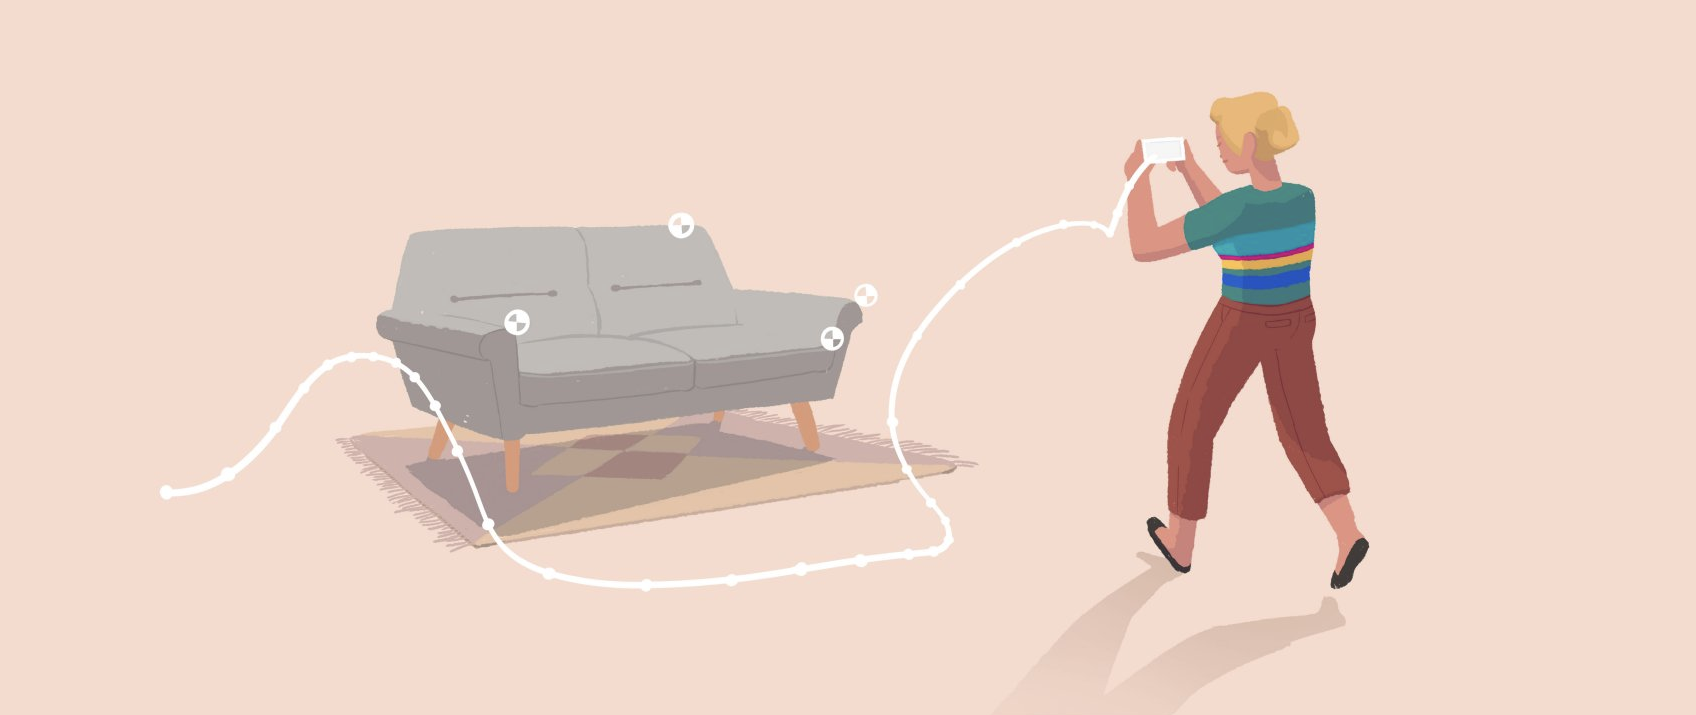
\includegraphics[width=15cm,height=5cm,keepaspectratio]{2Grundlagen/Bilder/motionTracking.png}
    \caption{Skizze zur Bewegungsverfolgung des Smartphones \cite{arcoreofficial.2020j}}
    \label{pic:motiontracking}
\end{figure}
\\ 
Die \acl{IMU} in Smart-Devices besitzt drei Beschleunigungssensoren, z.B. piezoelektrische Beschleunigungssensoren oder \ac{MEMS}, für die 
drei Raumachsen:
\begin{itemize}
    \item Die Abszissenachse (X-Achse), die horizontale (waagerechte) Koordinatenachse,
    \item Die Ordinatenachse (Y-Achse), die darauf vertikale (senkrechte) Koordinatenachse und
    \item Die Applikatenachse (Z-Achse), die auf beiden anderen Achsen senkrechte Achse \cite{koordinatennorm.1973m}
\end{itemize}
Ebenso besitzt die \acs{IMU} Drehratensensoren, z.B. ein Gyroskop zur Messung der Rotationsgeschwindigkeit, welche die Drehraten um 
diese Raumachsen messen. Durch die kontinuierliche Auslesung der Sensordaten, wird die Position des Geräts berechnet und in Form von 
drei Koordinaten ausgegeben. Ausgehend von dem Referenzkoordinatensystem wird die Position neu bestimmt. Die Abbildung \ref{pic:Positionsberechnung} 
veranschaulicht solch ein Beispiel.
\begin{figure}[hbt!]
    \centering
    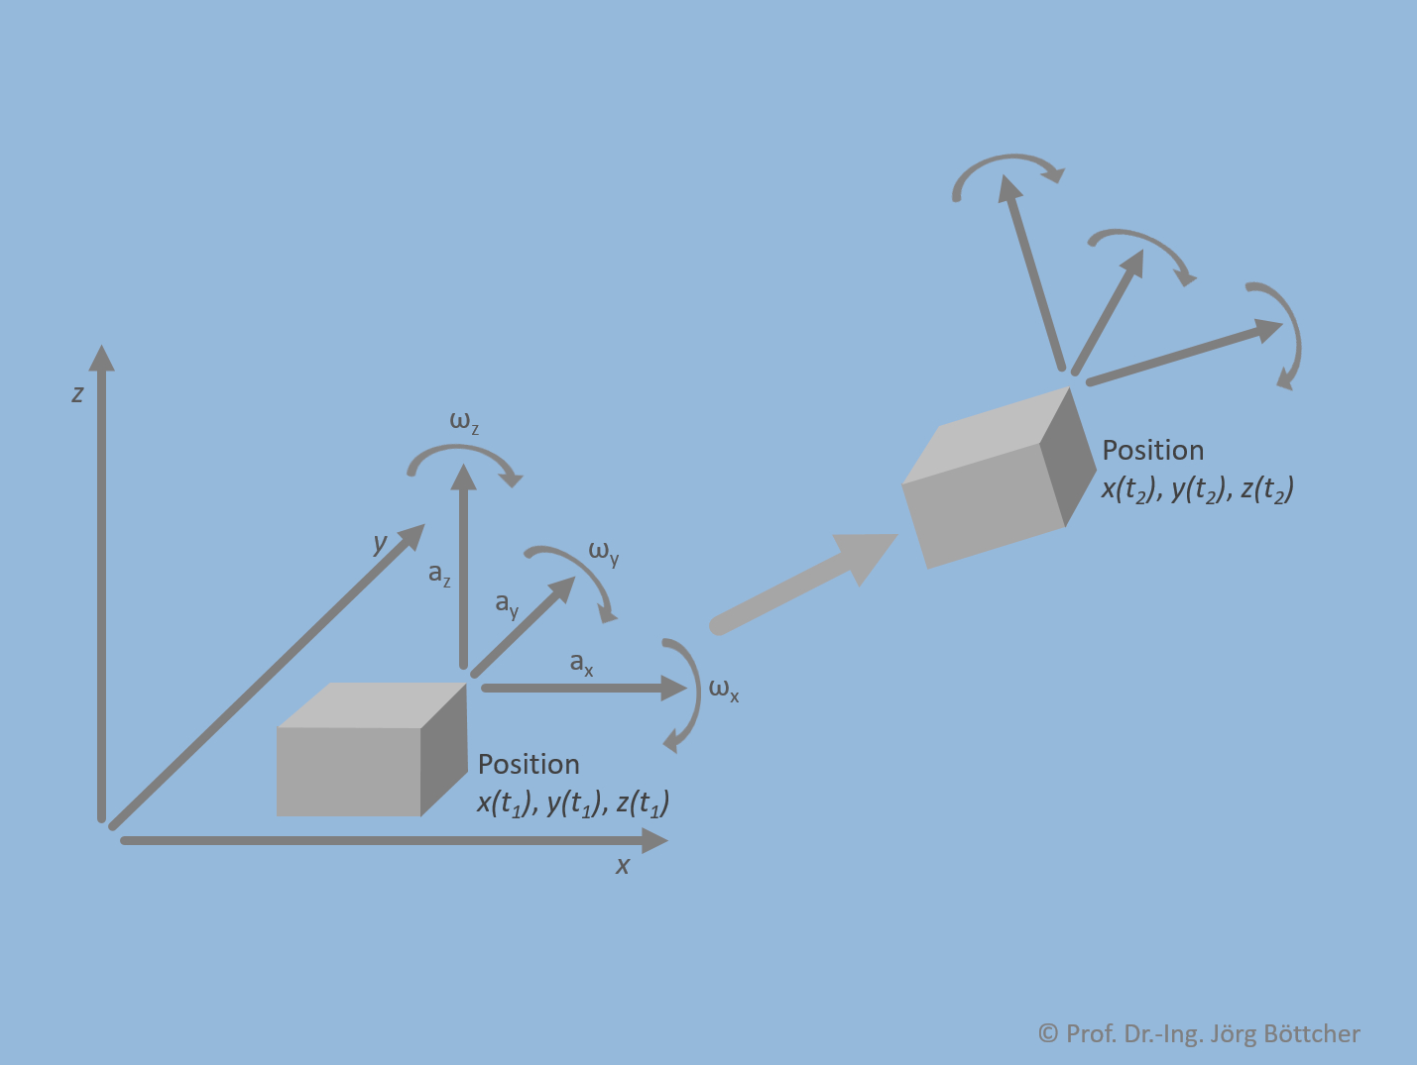
\includegraphics[width=9cm,height=9cm,keepaspectratio]{2Grundlagen/Bilder/imu-Bsp.png}
    \caption{Grundprinzip einer IMU \cite{imubild.2020j}}
    \label{pic:Positionsberechnung}
\end{figure}
\pagebreak
\subsubsection*{Environmental understanding}
Die zweite Schlüsselfunktion des Frameworks ist das Verständnis der Umgebung. Dieses wird erlangt, indem \textit{„feature points“}, Ebenen und 
Flächen beim Scannen des Umfelds erkannt werden. Beim Entstehen mehrerer solcher \textit{feature points} erstellt ARCore ein Cluster aller 
naheliegenden Punkte. Dieses erzeugte Cluster repräsentiert eine horizontale oder vertikale Fläche. Mit diesen gewonnenen Informationen ist das 
Platzieren von virtuellen Objekten auf den erfassten Flächen möglich.
\begin{figure}[hbt!]
    \centering
    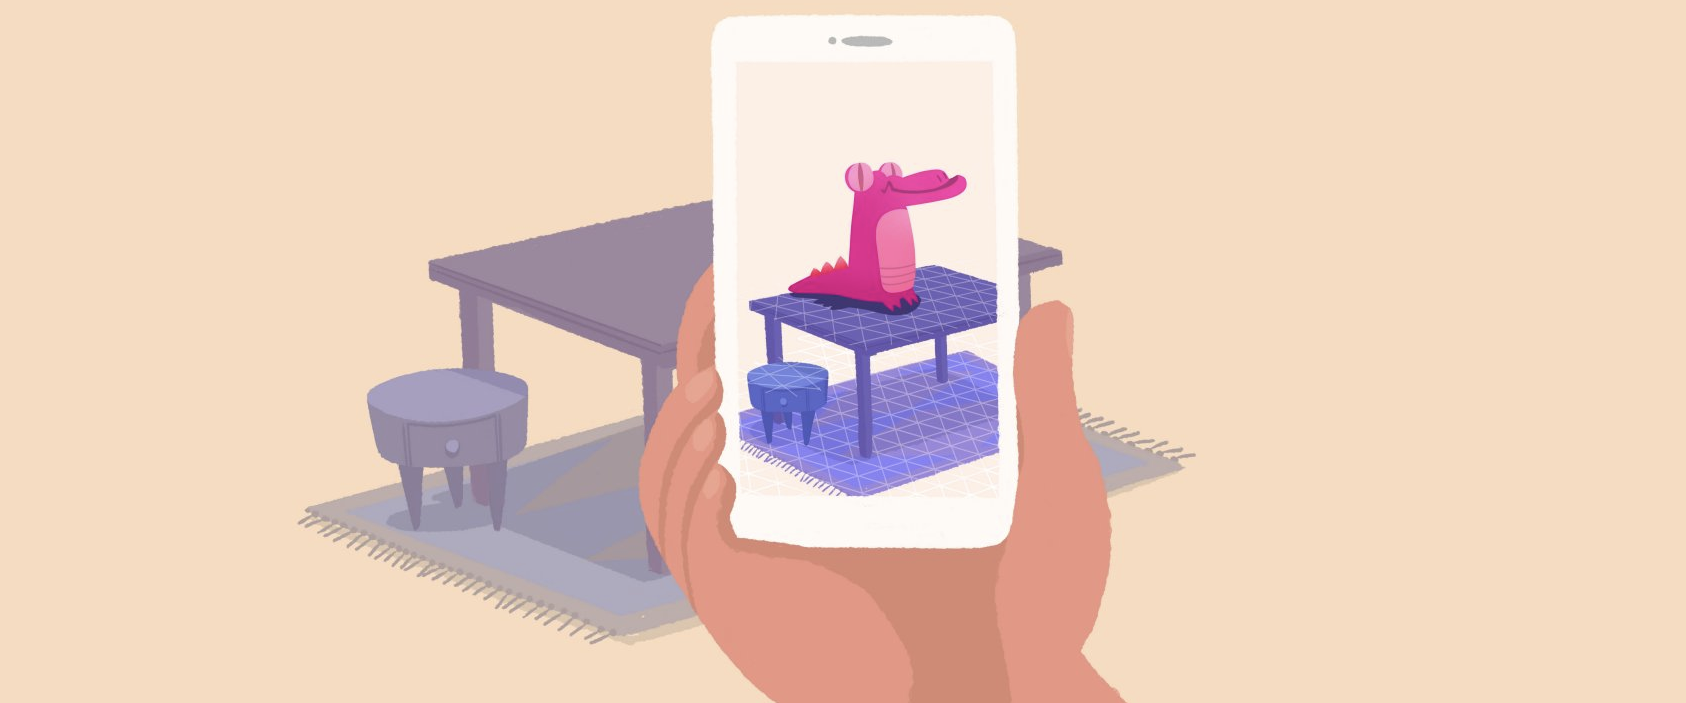
\includegraphics[width=15cm,height=5cm,keepaspectratio]{2Grundlagen/Bilder/environmentalUnderst.png}
    \caption{Skizze zum Umgebungsverständnis des Smartphones \cite{arcoreofficial.2020j}}
    \label{pic:environmentalunderst}
\end{figure}
\subsubsection*{Light estimation}
Mit der Funktion der Lichtschätzung kann ARCore Lichtverhältnisse und Informationen über die Beleuchtung der Umgebung erkennen. Dadurch kann das 
\acs{SDK} durchschnittliche Intensität und eine angepasste Farbkorrektur eines bestimmten Kamerabildes liefern, um so die Aufarbeitung des Bildes 
der Umgebung anzupassen. Diese Funktion verstärkt die Anpassung des virtuellen Objektes an die Realität und lässt dieses noch glaubwürdiger 
erscheinen.
\begin{figure}[hbt!]
    \centering
    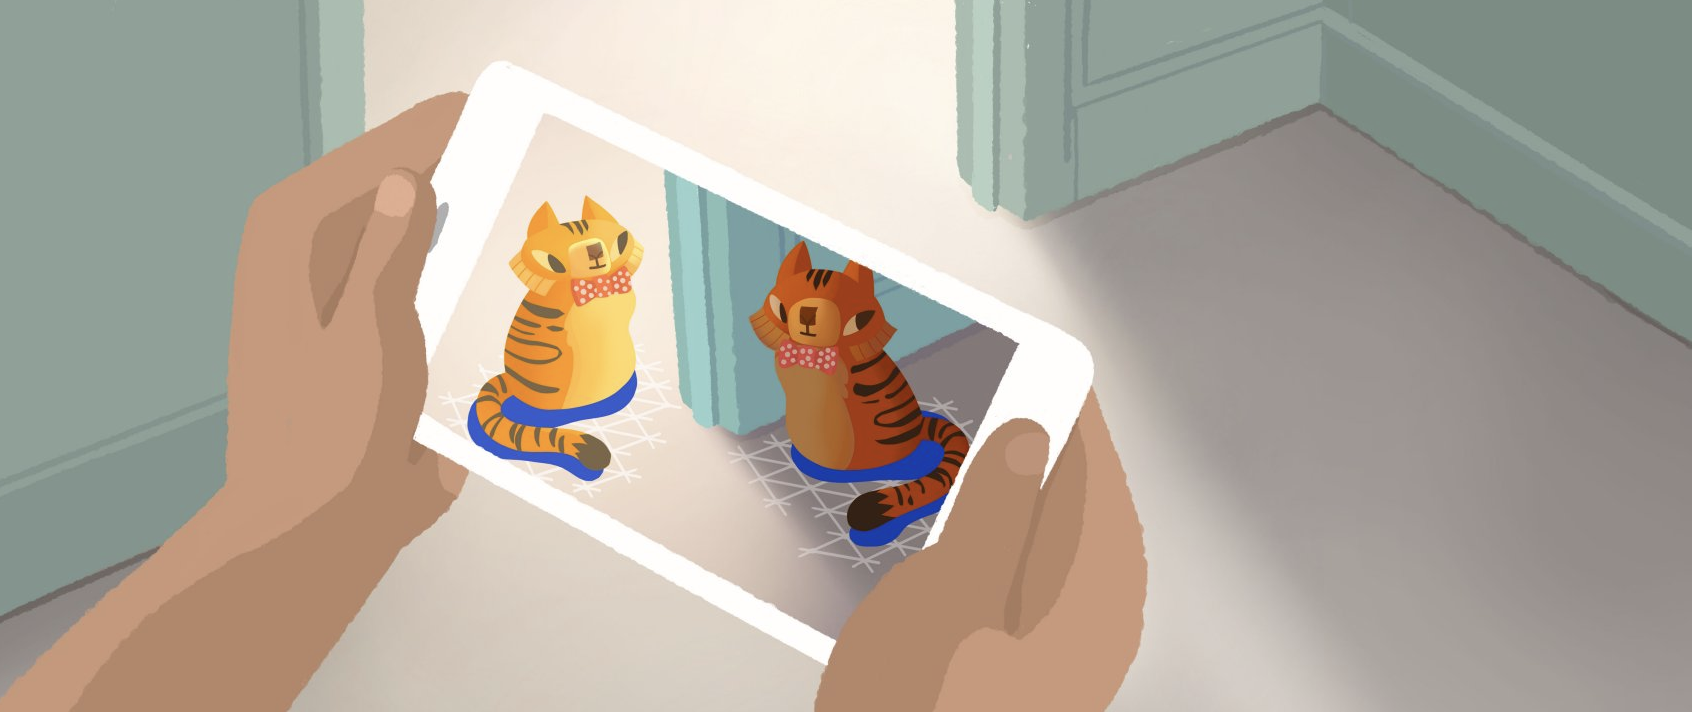
\includegraphics[width=15cm,height=5cm,keepaspectratio]{2Grundlagen/Bilder/lightEstim.png}
    \caption{Skizze zu den Lichtverhältnissen des Smartphones \cite{arcoreofficial.2020j}}
    \label{pic:lightestim}
\end{figure}
\subsection{Android Jetpack}
\label{sec:androidjetpack}
Android Jetpack ist eine Ansammlung an Bibliotheken, die es Entwicklern ermöglicht \textit{Best Practices} zu befolgen, 
Boilerplate\footnote{Sind Codeabschnitte, die an mehreren Stellen mit wenigen oder gar keinen Änderungen aufgeführt sein müssen. \cite{boilerplate.2019m}}-Code 
zu reduzieren.
%und Quell-/ Source-Code zu schreiben.
Die durch Android Jetpack zur Verfügung gestellten Bibliotheken fördern die konsistente Funktionsweise der 
Android-Versionen und -Geräten. Darüber hinaus wird mit Android Jetpack ein Überblick verschafft, um Best Practices und empfohlene 
Architekturen zu berücksichtigen.
\\ 
Außerdem wurde Android Jetpack für moderne Design-Praktiken entwickelt, darunter fällt \textit{„seperation of concerns“}\footnote{(SoC), Entwurfsprinzip, um verschiedene Verantwortlichkeiten auf 
verschieden Abschnitte zu trennen. \cite{soc.2019a}}, \textit{testability}, \textit{loose coupling}, \textit{Observer Pattern}\footnote{Beobachter-Muster, Verhaltensmuster der GoF-Muster}, 
\textit{Inversion of Control}\footnote{(IoC), Umsetzugsparadigma, das ein spezifisches Objekt über ein mehrfach verwendetes Objekt aufruft. \cite{ioc.2020}} und 
\textit{productivity features}, z.B. Plugin-Integrationen. Dies sind Techniken, um eine robuste und qualitativ hochwertige App zu erstellen.
\\ 
Die Bibliothekensammlung ist die Grundlage für die verwendete Architektur, Android Architecture Components in Abschnitt \ref{chap:AAC}.
\\ 
\linebreak
Die Abbildung \ref{pic:androidjetpackcomp} zeigt einen Überblick über die in Jetpack enthaltenen Bibliotheken. % in Abschnitt \ref{chap:AAC}
\begin{figure}[hbt!]
    \centering
    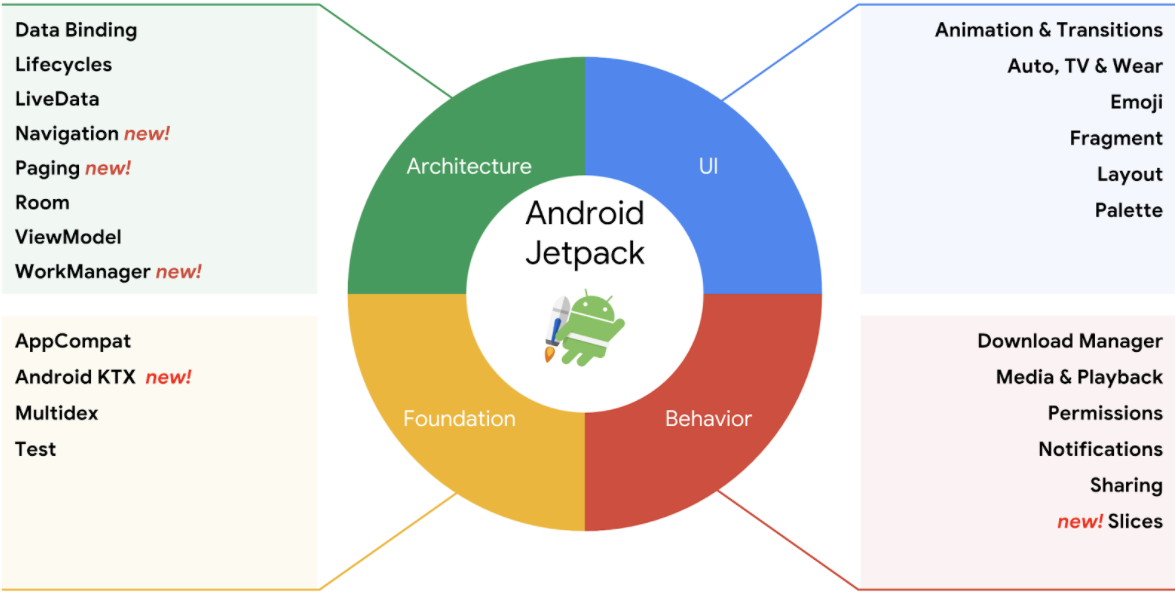
\includegraphics[width=15cm,height=10cm,keepaspectratio]{2Grundlagen/Bilder/androidjetpackcomps.png}
    \caption{Komponenten von Android Jetpack \cite{androidjpdescr.2018m}}
    \label{pic:androidjetpackcomp}
\end{figure}
\\
Eine nähere Erläuterung aller Bibliotheken findet im Rahmen dieser Ausarbeitung nicht statt, wobei die zur Verwendung geplanten 
„Architecture Components“ beschrieben werden. 
\\ 
\linebreak
LiveData, Room und ViewModel sind Bestandteil der \textit{Android Architecture Components}-Konstellation 
und bilden die Basis für die Architektur, welche an das \textit{MVVM-Pattern} angelehnt ist.

\subsection*{LiveData}
\label{sec:LiveData}
\textit{LiveData} gehört zu den \textit{Observer-Pattern} und ist eine Datenhalterklasse die eine Beobachtungsfunktion, bzw. -charakter besitzt. Der 
Unterschied zu einem regulären Observable ist, die lebenszyklus-unabhängige LiveData-Komponente. Dies bedeutet, der Lebenszyklus anderer 
Komponenten z.B. \textit{Activities, Fragments oder Services}, wird berücksichtigt. Mit dieser Kenntnis wird sichergestellt, dass LiveData 
nur App-Komponenten beobachtet, welche sich in einem aktiven Lebenszyklus befinden.
\\ 
\linebreak
Vorteile die die \textit{LiveData}-Komponente mit sich bringt sind unter anderem die Sicherstellung der Übereinstimmung der Benutzeroberfläche und 
deren Datenstatus, vorbeugend gegenüber Speicherverlust, immer auf dem aktuellsten Stand der gespeicherten Informationen und der Wegfall 
der manuellen Lebenszykluskoordination. \cite{livedata.2020}
\subsection*{Room}
\label{sec:Room}
\textit{Room} ist eine Persistenzbibliothek und bietet ein Abstraktionsschicht über der eigentlichen \textit{\acs{SQL}ite}-Datenbank, um einen 
robusten Datenbankzugriff zu managen und das volle Potential von \acs{SQL}ite gleichzeitig zu nutzen. \cite{room.2017}
\\ 
\linebreak
Die robuste \acs{SQL}-Objektzuordnungsbibliothek \textit{Room} kann einen Cache mit den Daten der Applikation auf einem Gerät erstellen. Dieser 
Cache dient als Wahrheitsquelle der Applikation und ermöglicht den Benutzern eine konsistente Kopie der Informationen der App anzuzeigen 
und immer zugänglich zu machen. \textit{Room} kann in drei Kategorien, bzw. in drei Hauptkomponenten unterteilt werden:
\begin{itemize}
    \item Room database: Dient als Zugriffspunkt für die zugrundeliegende SQLite-Datenbank
    \item DAO (Data Access Object): Beinhaltet Methoden um Datenbankzugriffe zu gewährleisten.
    \item Entity: Repräsentiert ein Objekttabelle der Datenbank.
\end{itemize}
Das Diagramm \ref{pic:roomarchitecturediagramm} veranschaulicht die Interaktion, bzw. Funktionsweisen der Hauptkomponenten.
\begin{figure}[hbt!]
    \centering
    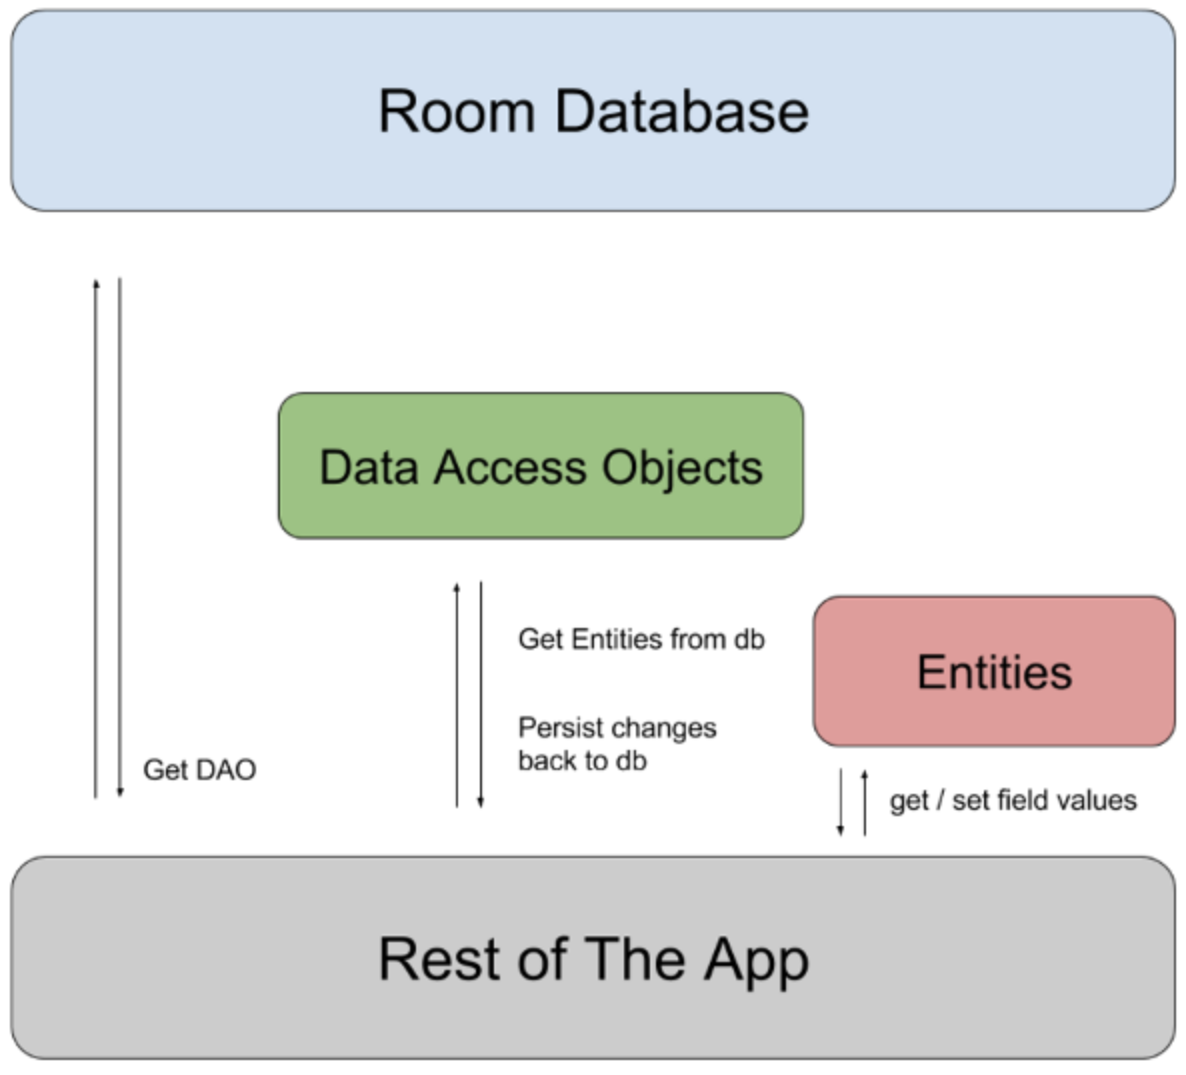
\includegraphics[width=7.5cm,height=7.5cm,keepaspectratio]{2Grundlagen/Bilder/roomArchitecture.png}
    \caption{Room Architektur Diagramm \cite{roomdiagr.2017}}
    \label{pic:roomarchitecturediagramm}
\end{figure}
\\ 
%\pagebreak
\linebreak
Allgemein ermöglicht \textit{Room} einen vereinfachten Zugriff auf die Datenbank. Die Bibliothek hat einen hohen Grad an Möglichkeiten der \textit{„testability“}. 
Zur Kompilierungszeit wird eine \acs{SQL}-Abfrageüberprüfung durchgeführt und interagiert einwandfrei mit anderen Android Architecture 
Components, z.B. LiveData und ViewModel.

\subsection*{ViewModel}
\label{sec:ViewModel}
Grundsätzlich dient das \textit{ViewModel} als lebenszyklusbewusste Speicherung und Verwaltung von benutzeroberflächenbezogenen Daten. 
Durch die \textit{ViewModel}-Klasse können Informationen Konfigurationsänderungen, z.B. Bildschirmdrehungen, die als Änderung zählen, 
überstehen. Eine Konfiguration kann sog. Activities verwerfen und neu laden, so können nicht persistierte Daten verloren gehen. 
\\ 
\linebreak
Ein \textit{ViewModel} fungiert ebenso als Kommunikationsschnittstelle zwischen den darüber- und darunterliegenden Komponenten der 
Architektur (siehe Abschnitt \ref{chap:AAC}). Des Weiteren kann die \textit{ViewModel}-Komponente Informationen zwischen Benutzeroberflächen 
und verschiedenen Fragmenten, engl. \textit{„fragments“}\footnote{Teil einer \ac{UI} in einer Android Activity}, teilen.
\\ 
\linebreak
Die Abbildung \ref{pic:viewModeldiagramm} zeigt eine sich ändernde Activity, die zu Beginn und nach Neuerstellung oder Aktualisierung Zugriff 
auf die unveränderten Daten hat. 
\begin{figure}[hbt!]
    \centering
    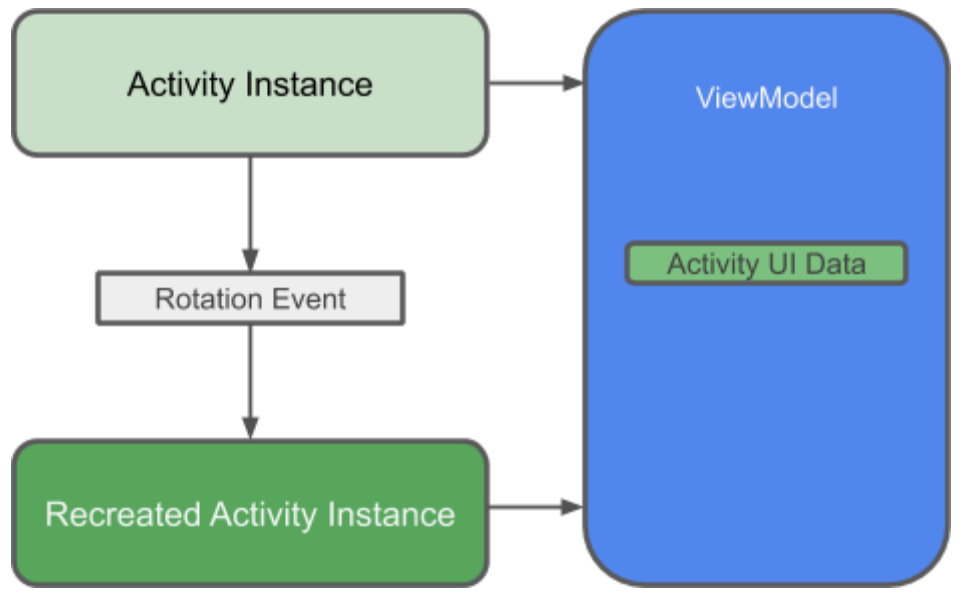
\includegraphics[width=7.5cm,height=7.5cm,keepaspectratio]{2Grundlagen/Bilder/viewModelDiagram.png}
    \caption{ViewModel Struktur Diagramm \cite{viewmodeldiagr.2020}}
    \label{pic:viewModeldiagramm}
\end{figure} 
\pagebreak
\subsection{Sceneform SDK}
Das Sceneform \acs{SDK} ist ein Open-Source Projekt der Google LLC., welches für das Rendern von 3D-Szenen und -Animationen zuständig ist. 
Basierend auf der physikalischen Echtzeit-Rendering-Engine, \textit{physically based renderer} für Android, iOS, macOS, Linux und Windows 
von Google Filament, wurde Sceneform entwickelt. 
\\ 
\linebreak
Bei dem Ansatz des physikalisch basierten Renderns in der Computergrafik wird versucht, alle Modalitäten der realen Welt genauer zu modellieren. 
Mit dieser Methode werden virtuelle 3D-Objekte in der \acl{AR} noch realer dargestellt, um einen Echtheitseffekt zu erzielen und zu simulieren. 
Ein Beispiel ist das Simulieren des Lichtflusses, um einen Schatten des Objekts zu erzeugen, wodurch die Wirksamkeit immer mehr der Realität 
entspricht.
\\ 
\linebreak
Dreidimensionale Modelle werden als \textit{(.obj)}-Dateien in das Projekt importiert. Diese Dateien beinhalten aufgelistete Punkte, Vektoren 
und Linien, welche das Modell repräsentieren. Das \textit{Sceneform \acs{SDK}} verwendet die \textit{.obj}-Datei und konvertiert, bzw. 
rendert diese in eine, \textit{Sceneform binary assets (.sfb)}-Datei. Diese generierte Datei ermöglicht das Generieren eines dreidimensionalen 
Objekts, welches anschließend in \acs{AR}-Anwendungen basierend auf Google ARCore verwendet werden kann. 
Für die finale Renderung und Anzeige ist die \textit{ModelRenderable}-Klasse des \acs{SDK}s zuständig. 
%\\ 
%\linebreak
%Ein weiterer wichtiger Aspekt diese Projekts ist der Einsatz einer Datenbank, um generierte Daten speichern zu können.
\subsection{SQLite}
\acs{SQL}ite ist eine Open-Source In-Process-Bibliothek, die ein in sich geschlossenes, serverloses, transaktionsfreies \acs{SQL}-Datenbankmodul 
ohne Konfiguration implementiert. \acs{SQL}ite ist eine eingebettete \acs{SQL}-Datenbank-Engine die im Gegensatz zu anderen \acs{SQL}-Datenbanken über 
keinen separaten Serverprozess verfügt, d.h. Transaktionen, Lese- und Schreibzugriffe werden direkt auf eine normale Festplattendatei getätigt. \cite{sqlite.2018j}
\\
Darüber hinaus ist \acs{SQL}ite plattformübergreifend und kann beliebig Datenbank- und Objekttabellen, Indizes und Ansichten erstellen und verwalten. 